%----------------------------------------------------------------------------------------
%	Einleitung
%----------------------------------------------------------------------------------------

\chapter{Einleitung}
\label{ch:einleitung}

\section{Problemstellung}
Die forensische Analyse von digitalen Beweismitteln ist in der heutigen Zeit ein wichtiger Aspekt, um in der Strafverfolgung rechtswidriges Verhalten aufzudecken oder nachzuweisen. In vielen Fällen werden informationstechnische Systeme am Tatort gefunden oder zur Tatbegehung genutzt. Einschlägig sind hierbei Angriffe auf kritische Infrastrukturen durch Computersabotage oder das Ausspähen von Daten. Aber auch Urheberrechtsverletzungen durch die Weitergabe von geschützten Medien oder Verstöße gegen das Wettbewerbsrecht werden mit Informationstechnik begangen.
Je nach Dauer und Umfang der Strafhandlung werden gerade auch im Bereich der Wirtschaftskriminalität dutzende Asservate von informationstechnischen Systemen sichergestellt. Beispielsweise werden beteiligte Computer und Mobiltelefone beschlagnahmt. Oder es werden logische Sicherungen von Netzwerkspeichern durchgeführt.\\

\noindent
Bei der Analyse dieser Asservate möchte ein forensischer Ermittler möglichst schnell einen Überblick über die sichergestellten Daten erhalten. Darauf aufbauend kann er entscheiden, welche Spuren in den Daten zum Nachweis konkreter Tathandlungen dienen und welche potentielle Beweismittel nicht weiter analysiert werden müssen.\\

\noindent
Der kritischste Aspekt hierbei ist, in kürzester Zeit die richtigen Informationen aus allen Daten zu extrahieren. Denn gerade in der Strafverfolgung ist eine schnelle und zielgerichtete Aufarbeitung der Ermittlungsfälle erforderlich. Darüber hinaus werden während der Analyse oftmals weitere Indizien gefunden, welche wiederum zur Sicherung neuer Asservate führen können. Je mehr Zeit jedoch für die Analyse benötigt wird, desto höher ist die Gefahr, dass noch nicht sichergestellte Daten endgültig gelöscht werden. Beispielsweise werden Telekommunikationsverbindungsdaten nicht über längere Zeiträume gespeichert.\\

\noindent
Zur Analyse stehen dem Forensiker etliche proprietäre und Open-Source Programme zur Auswahl. Allerdings sind im forensischen Open-Source Bereich viele Programme durch die Ressourcen des Analyserechners beschränkt. Sie bieten keine Möglichkeiten rechenintensive Aufgaben performant auf mehreren Computern zu skalieren.\\

\noindent
Aus fachlicher Sicht wäre eine Plattform sinnvoll, die anfallende Analyseaufgaben automatisiert auf allen Daten durchführt. Das System sollte die Ergebnisse, unter Berücksichtigung verfügbarer Ressourcen, schnellstmöglich ermitteln und dem forensischen Ermittler in einer aufbereiteten Form darstellen. Auf Basis dieser Ergebnisse kann sich der Forensiker möglichst frühzeitig einen Überblick über alle Asservate verschaffen, um dann bestimmte Daten auch in anderen spezialisierten Analyseanwendungen weiterzuverarbeiten. 

\section{Zielsetzung}
Zur Lösung der Problemstellung soll in dieser Masterthesis eine Plattform zur forensischen Analyse entwickelt werden. Diese Plattform soll durch eine automatisierte Analyse und Aufbereitung forensisch relevanter Informationen dem Forensiker helfen, sich einen Überblick zu verschaffen. Er soll dadurch effizient und zielgerichtet Datenanalysen durchführen können. Als Basis dieser Plattform soll das Apache Hadoop\textsuperscript{\textregistered} Framework genutzt werden. Hierbei sollen Vor- und Nachteile dieser Art der Datenverarbeitung im forensischen Kontext herausgearbeitet werden.\\ 

\noindent
Apache Hadoop ist ein etabliertes Open-Source Framework zur verteilten Speicherung und Verarbeitung von Daten. Durch die parallele Datenverarbeitung eignet sich ein Hadoop-Cluster auch zur Prozessierung von großen Datenmengen im Terabyte-Bereich. Ein zugrunde liegendes Paradigma ist hierbei, dass die Programmausführung dort stattfindet, wo auch die Daten liegen, um kostspielige Datentransporte weitgehend zu vermeiden. Aufgrund dieser Beschaffenheit kann diese Art der Datenverarbeitung auch Geschwindigkeitsvorteile bei forensischen Analysen bieten. \\

\noindent
Ein wichtiger Aspekt der Masterthesis ist die Aufbereitung der Daten für die Analyse im Hadoop-Cluster. Hierbei sollen mehrere Möglichkeiten analysiert werden, wie diese Aufbereitung und Speicherung der Daten im Hadoop-Cluster gelingen kann. Dabei muss auch auf die Unversehrtheit der Dateiinhalte und Metadaten bei der Aufbereitung geachtet werden. Darauf aufbauend soll eine fachliche Verwaltungsstruktur entwickelt werden, die es auch erlaubt, mehrere Asservate von beliebigen Ermittlungen parallel zu verarbeiten. Dadurch können auch Zusammenhänge zwischen unterschiedlichen Asservaten identifiziert werden.\\

\noindent
Im Rahmen der Thesis soll die Datenanalyse vorerst grundlegende Funktionen unterstützen.
So sollen die Metadaten, wie beispielsweise Name, Dateipfad, Hashsumme, Dateityp, Größe und Zeitstempel ermittelt werden und zu weiteren Analysen zur Verfügung stehen.
Es soll auch eine Volltextsuche auf den Daten möglich sein. Darauf aufbauend soll der Nutzer beispielsweise gleiche Dateien und Verbindungen zwischen den einzelnen Beweismitteln erkennen können.
Optional könnte die Analyseplattform gezielt nach IP-Adressen, Web-Adressen, E-Mail-Adressen oder Positionsdaten\footnote{Beispielsweise könnten Geopositionen oder Ortsnamen aus Dateien extrahiert werden. Diese Daten könnten dann mit ihrem geografischen Bezug auf einer Karte dargestellt werden.} suchen.\\

\noindent
Die Resultate durchgeführter Datenanalysen sollen dem Nutzer bereitgestellt werden. Hierzu
wird eine grafische Oberfläche benötigt, welche die fachlichen Aspekte der forensischen Analyseplattform widerspiegelt. Im Rahmen der Thesis sollen Möglichkeiten analysiert werden, wie eine grafische Oberfläche aussehen könnte. In diesem Kontext soll auch geprüft werden, ob existierende Programme zur Datenvisualisierung im Hadoop-Umfeld wiederverwendet werden können. Die Implementierung einer grafischen Oberfläche ist im Rahmen dieser Thesis jedoch nicht angedacht.\\

\noindent
Abbildung \ref{fig:foam_analysis_approach} skizziert das angestrebte Analysevorgehen mit dieser Analyseplattform. Der Forensiker soll digitale Asservate in das Hadoop-Cluster importieren können. Nachfolgend hat er die Möglichkeit, diverse Analysen auf den Daten durchzuführen. Die Ergebnisse könnten später über eine entsprechende Oberfläche visualisiert werden.\\

\begin{figure}[ht]
  \centering
  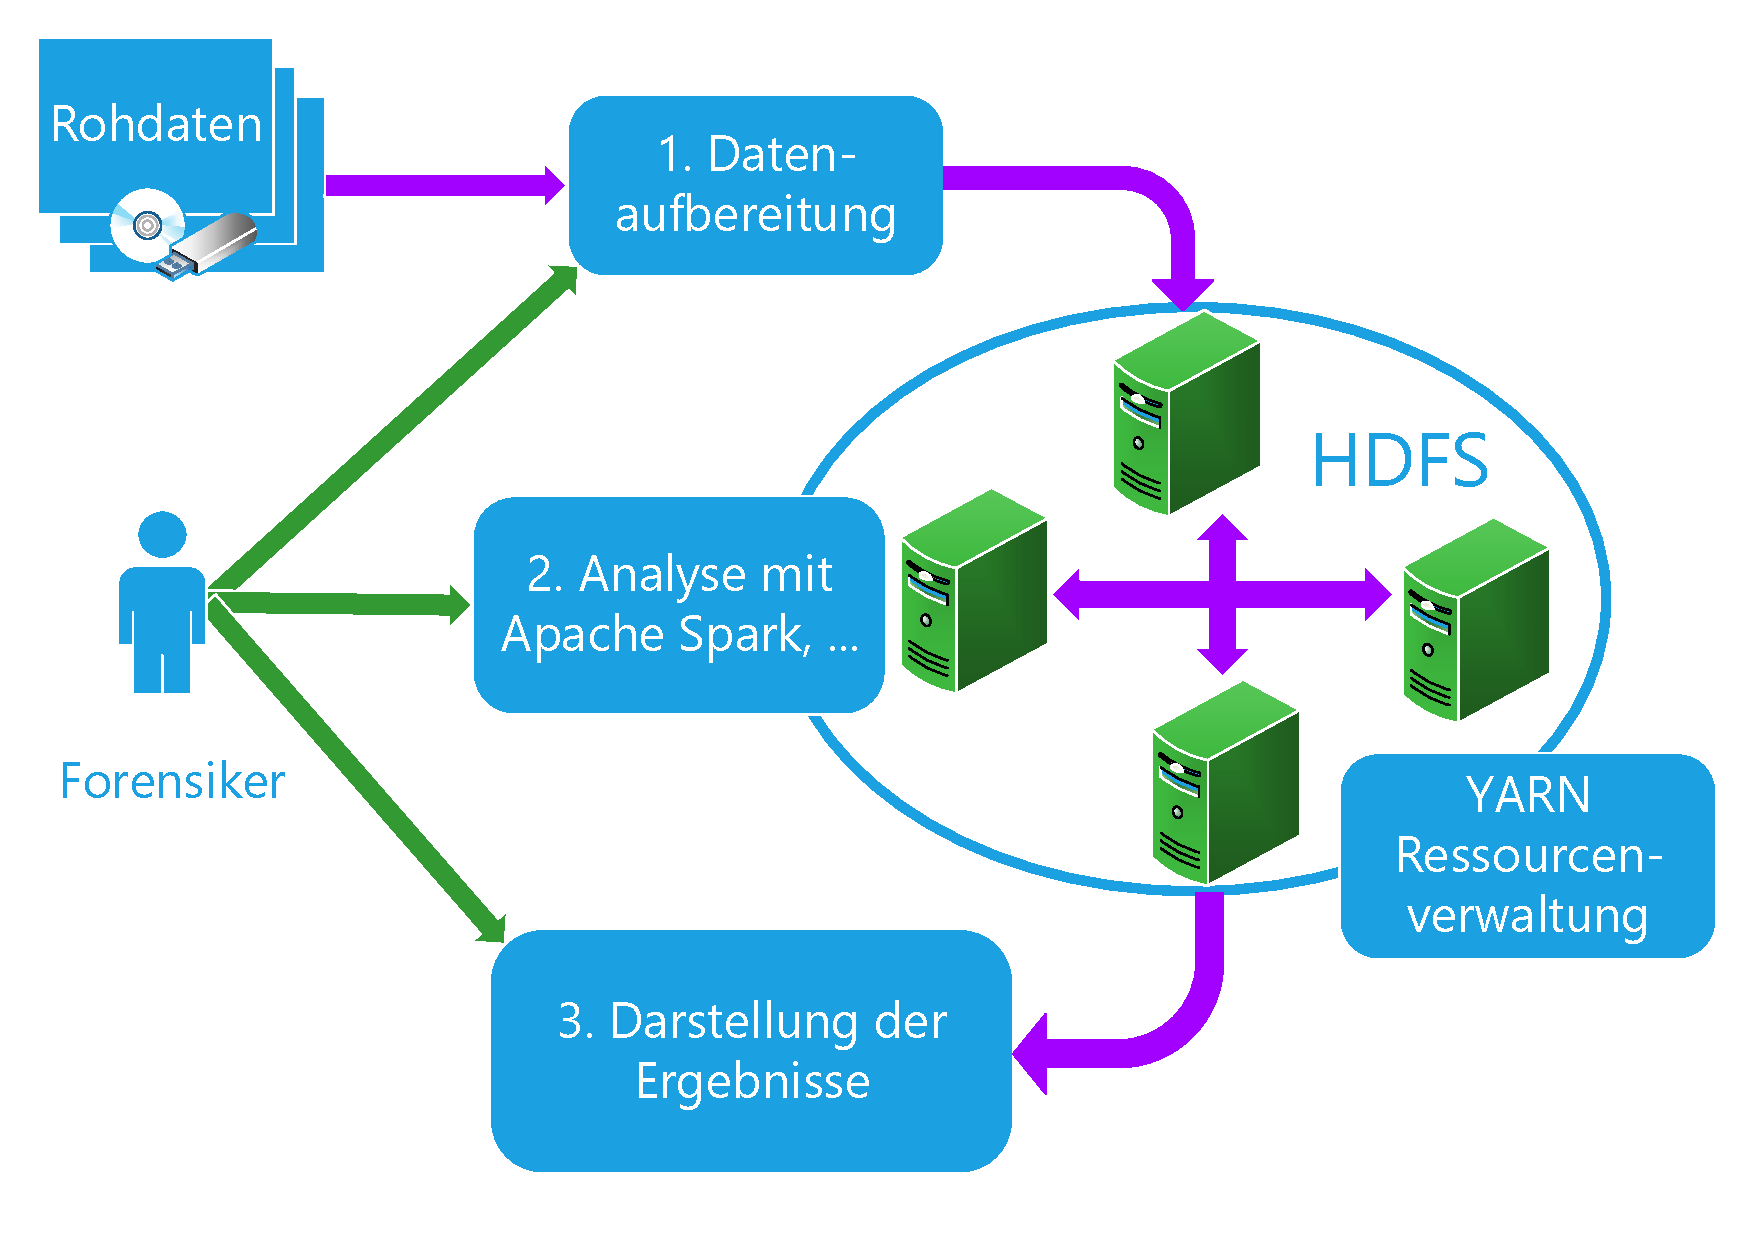
\includegraphics[width=0.82\textwidth]{./resource/Hadoop-Struktur.pdf}
  \caption{Analysevorgehen}
  \label{fig:foam_analysis_approach}
\end{figure}

\noindent
Das Ziel dieser Masterthesis ist es, dem forensischen Ermittler schnellstmöglich einen Überblick zu den einzelnen Beweismitteln und deren Zusammenhänge im Kontext einer Fallanalyse zu liefern. \\

\noindent
Bei einer realen forensischen Analyse gibt es weitere Anforderungen, die das Analysesystem erfüllen sollte. Da in vielen Fällen hochsensible personenbezogene Daten und Geschäftsgeheimnisse verarbeitet werden, müssen auch entsprechende Regelungen getroffen werden, wie nach der Analyse alle Daten restlos aus dem System gelöscht werden können.\\
Das System muss gegen fremden Zugriff gesichert sein. Es muss zu jeder Zeit ersichtlich sein, welche Personen zu welchem Zweck auf das System zugreifen.\\
Ein weiterer Aspekt in der Analyse ist die lückenlose Erstellung einer Beweismittelkette (Chain of Custody). Für jedes forensische Analyseergebnis müssen die Herkunft und die Verarbeitungsschritte transparent nachvollziehbar sein.\\
Im Rahmen der Masterthesis sollen diese Aspekte zumindest theoretisch und wenn möglich, auch praktisch analysiert werden.\\

\noindent
Aus organisatorischer Sicht soll die Analyseplattform als Open Source Projekt bereitgestellt werden. Hierzu soll der Source-Code, die Konfiguration des Systems und die Dokumentation in einer öffentlich zugänglichen Versionsverwaltung verfügbar sein.\\


\clearpage
\section{Aufbau}
In Kapitel \ref{ch:einleitung} wird das Eingangsproblem und die Ziele dieser Masterthesis beschrieben.\\ 

\noindent
In Kapitel \ref{ch:development_approach} folgt das allgemeine Entwicklungsvorgehen. Darin ist der aktuelle Projektplan enthalten, welcher die Arbeitspakete definiert.
Zusätzlich wird die genutzte Entwicklungsumgebung skizziert.\\

\noindent
In Kapitel \ref{ch:theory_hadoop} erfolgt eine Darstellung der Apache Hadoop Plattform, inklusive der theoretischen Grundlagen zur Arbeitsweise des Frameworks. Des Weiteren werden darauf aufbauende Projekte, wie beispielsweise Apache Spark und Apache HBase erklärt.\\

\noindent
In Kapitel \ref{ch:data_persistence} werden unterschiedliche Varianten zur Datenspeicherung und Aufbereitung analysiert. Innerhalb dieses Kapitels wird ein Vorgehen entwickelt, wie die Daten eines Asservats im Hadoop-Cluster gespeichert werden können, um sie später parallelisiert verarbeiten zu können. Zu Beginn wird das herkömmliche Analysevorgehen in Verbindung mit der Analyseanwendung \textit{Autopsy} beschrieben, um fachlich relevante Aspekte bei der Analyse herauszuarbeiten.\\

\noindent
Die eigentliche Datenverarbeitung wird in Kapitel \ref{ch:data_processing} beschrieben. Hier wird ein Ansatz vorgestellt, wie die Daten parallel verarbeitetet werden können. Anhand dieses Ansatzes werden Hashsummen der Daten berechnet und die Medientypen der Dateien ermittelt. Zum Schluss wird eine Möglichkeit vorgestellt, wie die Informationen für eine Volltextsuche aufbereitet werden können.\\



\noindent
Die Visualisierung der Informationen ist ein interessanter Aspekt der forensischen Analyseplattform, welcher in Kapitel \ref{ch:data_visualization} beschrieben wird. Dort werden einige Möglichkeiten erläutert, wie eine Visualisierung aussehen könnte.\\

\noindent
In Kapitel \ref{ch:additional_aspects} werden querschnittliche Aspekte zur Datensicherheit von forensischen Analysen und zum Löschen von Daten dargestellt.\\

\noindent
Zuletzt erfolgt in Kapitel \ref{ch:zusammenfassung} eine Zusammenfassung der erarbeiteten Ergebnisse. Es wird auch aufgezeigt, ob das Apache Hadoop Framework überhaupt die Anforderungen einer forensischen Analyseplattform erfüllen kann.\\

\noindent
Offene Punkte und Verbesserungen werden in Kapitel \ref{ch:ausblick} beschrieben. 
